\documentclass[paper=a4, fontsize=11pt]{scrartcl} % A4 paper and 11pt font size
\usepackage[section]{placeins}
\usepackage[T1]{fontenc}
\usepackage[polish]{babel}
\usepackage[utf8x]{inputenc}
\usepackage{lmodern}
\selectlanguage{polish}
\usepackage{mathtools}
\usepackage{listings}   
\usepackage{enumerate}
\usepackage{tikz}
\usepackage{circuitikz}
\usepackage{graphicx}
\usepackage{dblfloatfix}
\usepackage{caption}
\usepackage{subcaption}
\usepackage{sectsty} % Allows customizing section commands
\allsectionsfont{\centering \normalfont\scshape} % Make all sections centered, the default font and small caps
\setlength\parindent{0pt} % Removes all indentation from paragraphs - comment this line for an assignment with lots of text

\begin{document}

\begin{titlepage}

\newcommand{\HRule}{\rule{\linewidth}{0.5mm}} % Defines a new command for the horizontal lines, change thickness here

\center % Center everything on the page
%----------------------------------------------------------------------------------------
%	HEADING SECTIONS
%----------------------------------------------------------------------------------------
\textsc{\LARGE Politechnika Warszawska}\\[1.5cm] % Name of your university/college
\textsc{\Large Wydział Elektroniki i Technik Informacyjnych}\\[0.5cm] % Major heading such as course name
\textsc{\large Praca dyplomowa inżynierska\\
na kierunku Informatyka\\
w specjalności Inżynieria Systemów Informatycznych}\\[0.5cm] % Minor heading such as course title

%----------------------------------------------------------------------------------------
%	TITLE SECTION
%----------------------------------------------------------------------------------------

\HRule \\[0.4cm]
{ \huge \bfseries Opracowanie programu do stereoskopowej wizualizacji detektora ALICE}\\[0.4cm] % Title of your document
\HRule \\[1.5cm]
 
%----------------------------------------------------------------------------------------
%	AUTHOR SECTION
%----------------------------------------------------------------------------------------

\begin{minipage}{0.4\textwidth}
\begin{flushleft} \large
\emph{Autor:}\\
Ahata \textsc{Valiukevich}
\end{flushleft}
\end{minipage}
~
\begin{minipage}{0.4\textwidth}
\begin{flushright} \large
\emph{Promotor:} \\
mgr inż. Julian \textsc{Myrcha} % Supervisor's Name
\end{flushright}
\end{minipage}\\[4cm]


%----------------------------------------------------------------------------------------
%	DATE SECTION
%----------------------------------------------------------------------------------------

{\large \today}\\[3cm] % Date, change the \today to a set date if you want to be precise
\vfill % Fill the rest of the page with whitespace
\end{titlepage}

\newpage

\section{Wstęp}
W przeciągu ostatnich kilku lat nauka zrobiła duży postęp w kierunku rozwoju fizyki dużych energii. Osiągnięcie to składa się z wyników dużej liczby badań oraz eksperymentów prowadzonych w różnych naukowo-badawczych instytucjach. Równolegle z naukami fizycznymi rozwiajała się również branża informatyczna, a w szczególności grafika komputerowa. Obecnie jest obserwowany coraz silniejszy trend związany z rozwojem technik stereoskopowych. Przy połączeniu badań fizycznych i grafiki komputerowej powstaje możliwość dogłębnego przestudiowania zjawisk zachodzących podczas rożnych eksperymentów.


\subsection{Cele i zakres pracy}
Pierwszym celem niniejszej pracy dyplomowej jest stereoskopwa wizualizacja detektora oraz zdarzeń ciężkich ionów w eksperymencie ALICE. Kolejnym istotnym celem pracy jest połączenie wyżej wymienionych wizualizacji do jednego spójnego obrazu. \\
Dla realizacji celi podstawowych niezbędne jest zapoznanie się z technologią stereoskopii i aktualnie dostępnymi rozwiązaniami,przestudiowanie podstaw działania eksperymentu ALICE oraz środowiska informatycznego w CERN. \\
Celem pośrednim danej pracy jest zapoznanie się z możliwościami biblioteki OpenGL, a także innymi uwarunkowaniami ważymi w aspekcie projektowanej aplikacji.
\newpage
\section{Teoria}
\subsection{Biblioteka OpenGL} 
	OpenGL (z angielskiego Open Graphics Library) jest potężnym systemem graficznym stanowiącym niejako pomost między programistą a sprzętem komputera. Biblioteka ta została stworzona przez firmę \textit{Silicon Graphics}, jednego z potentatów na rynku grafiki komputerowej.\\
	 Procedury OpenGL umożliwiają rendorowanie obiektów o rożnych poziomach skomplikowania zaczynając od prostego punktu geometrycznego, linii lub wypełnionego wielokąta do utworzenia najbardziej złożonej, zakrzywionej powierzchni, oświetlonej i odwzorowanej teksturą. OpenGL pozwala programistom na dostęp do prymitywów geometrycznych i obrazowych, list wyświetlania, przekształcania modelu, oświetlenia i teksturowania, antyaliasingu, mieszania i wielu innych funkcji. Wszystkie elementy stanu OpenGL - nawet treść pamięci tekstur i bufor ramki - można uzyskać za pomocą aplikacji OpenGL. Dany system obsługuje także aplikacje wizualizacji z obrazami 2D traktowanymi jako typy prymitywów, którymi można manipulować podobnie jak obiektami geometrycznymi 3D.\\
	Mimo że specyfikacja OpenGL definiuje konkretny ciąg przetwarzania graficznego, dostawcy platformy mają swobodę dostosowywania konkretnej implementacji OpenGL w celu osiągnięcia sprecyzowanych celów w zakresie kosztów i wydajności. Pojedyncze wywołania mogą być wykonywane na dedykowanym sprzęcie, uruchamiane jako procedury programowe w standardowym systemie CPU lub implementowane jako kombinacja zarówno dedykowanych procedur sprzętowych, jak i programowych. Ta elastyczność implementacji skutkuje ​​przyśpieszeniem renderowania, w dodatku jest powszechnie dostępna na wszystkich jednostkach od komputerów o niskich kosztach, po wysokiej klasy stacjach roboczych i superkomputerach.\\
\begin{figure}[h]
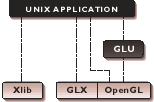
\includegraphics[width=6cm]{Hierarchy_UNIX.jpg}
\centering
\caption{Schemat ilustrujący relacje OpenGL GLU}
\end{figure}
\footnote{OpenGl podstawy wg https://www.opengl.org/about/}

\subsubsection{Shaders}
W OpenGL wszystko jest przedstawione w przestrzeni trójwymiarowej, ale na ekranie obraz widzimy listę pikseli 2D, w związku z tym duża część pracy OpenGL polega na zmianie współrzędnych 3D na piksele 2D, które by pasowały do ekranu. Cały proces transformacji jest zarządzany poprzez ciąg graficzny OpenGL. Ciąg przetwarzania może być podzielony na poszczególne kroki, gdzie na wejściu każdego kroku są wymagane dane wyjściowe poprzedniego. Każdy z tych kroków jest dobrze sprecyzowany, gdyż mają one konkretną funkcję, i może być wykonany równolegle. Większość współczesnych kart graficznych posiada setki, czasmi tysiące, małych jąder procesowych do szybkiego przetwarzania danych wejściowych. W ciągu graficznym dla przyśpieszenia przetwarzania uruchamiane są nieduże programy w GPU dla każdego kroku w ciągu. Wspomniane nieduże programy są nazywane \textit{\textbf{shaderami}}.\\
Shadery są pisane w języku w dużym stopniu podobnym do C - GLSL. GLSL jest dostosowany do wykorzystania w grafice, ponieważ zawiera przydatne funkcje skierowane na manipulacje wektorami i macierzami. Shadery zawsze zaczynają się od deklaracji wersji, następnie deklarowane są listy zmiennych wejściowych i wyjściowych, uniformy oraz ich główne funkcje. 
\paragraph*{Vertex shader.}
Pierwszym krokiem ciągu graficznego jest vertex shader, który jako daną wejściową przyjmuje jeden wierzchołek. Głównym celem vertex shadera jest transformacja współrzędnych 3D do innych współrzędnych 3D. Vertex shader również pozwala robić podstawowe przetwarzanie atrybutów wierzchołka.
\paragraph*{Primitive assembly.}
Primitive assembly jest krokiem, który za dane wejściowe przyjmuje wszystkie wierzchołki (lub jeden, jeśli wybrana jest flaga GL\_POINTS ) z vertex shadera. Na tym etapie przetwarzania kształtowane są prymitywy, wszystkie wierzchołki są grupowane do zadanego kształtu.
\paragraph*{Geometry shader}
Wyjście z primitive assembly jest przekazywane do geometry shadera. Geometry shader na wejściu przyjmuje kolekcję wierzchołków, które tworzą zadany kształt oraz mogą generować inne, emitując nowe wierzchołki, tworząc nowe (lub inne) prymitywy. 
\paragraph*{Rasterization.}
Dane wyjściowe geometry shadera są podawane na wejście etapu rasterization. W tym kroku uzyskane wcześniej prymitywy mapuje się na odpowiadające im piksele na ekranie ostatecznym. W wyniku czego powstają fragmenty do przetwarzania w kolejnym kroku, ale zanim zostanie uruchomiony fragment shader, jest wykonywane przycinanie. Przyciannie pozwala odrzucić wszystkie fragmenty, które są poza zasięgiem obserwatora, ów krok pozwala znacznie zwiększyć wydajność całego ciągu.
\textit{ Fragment w OpenGL zawiera wszystkie niezbędne dane do renderowania pojedynczego piksela.}
\paragraph*{Fragment shader.}
Głównym celem fragment shadera jest obliczenie końcowego koloru piksela i jest to zazwyczaj etap, na którym występują wszystkie zaawansowane efekty OpenGL. Z reguły fragment shader posiada wszystkie dane o scenie 3D (takie jak światła, cienie, kolor światła itp.), które można użyć do obliczania końcowego koloru piksela.

\subsubsection{GLFW} 
GLFW jest to Open Source, multipatformowa biblioteka dla OpenGL, OpenGL ES. Zapewnia ona proste API do tworzenia okien, kontekstów i powierzchni, odbierania danych wejściowych i zdarzeń. GLFW jest napisana w C posiada macierzystą obsługę systemów Windows, macOS i wielu systemów uniksopodobnych, takich jak Linux i FreeBSD. 
Zalety GLFW :
\begin{enumerate}
\item Tworzy okno i cały kontekst OpenGL używając wywołania tylko 2 funkcji.
\item Obsługuje OpenGL, OpenGL ES, Vulkan i powiązane opcje, flagi oraz rozszerznia.
\item Obsługuje wiele okien, wiele monitorów, ramp o wysokiej rozdzielczości DPI i gamma.
\item Obsługuje klawiatuę, mysz, gamepad, czas i okna zdarzenia, poprzez odpytywanie lub callback.
\item Dostęp do rodzimych obiektów i opcji kompilacji dla specyficznych funkcji platformy.
\end{enumerate} 

\subsubsection{GLEW}
The OpenGL Extension Wrangler Library (GLEW) jest wieloplatformową biblioteką C / C ++. GLEW zapewnia efektywne mechanizmy wykonawcze do określania, które rozszerzenia OpenGL są obsługiwane na docelowej platformie. Funkcje jądra i rozszerzenia OpenGL są widoczne w pojedynczym pliku nagłówkowym. GLEW została przetestowany na różnych systemach operacyjnych, w tym na systemach Windows, Linux, Mac OS X, FreeBSD i Solaris.
Podczas tworzenia wizualizacji została użyta wersja statyczna GLEW, czyli glew32s.lib. \footnote{http://glew.sourceforge.net/}

\subsubsection{GLM}
OpenGL Mathematics (GLM) jest nagłówkiem tylko do biblioteki matematycznej C++ dla oprogramowania graficznego opartego na specyfikacjach języka GLSL, udostępnia klasy i funkcje zaprojektowane i zaimplementowane z użyciem tych samych konwencji nazewnictwa jak w GLSL. Mimo to GLM nie jest ograniczony tylko do cech GLSL. System rozszerzenia, oparty na konwencjach rozszerzeń GLSL, zapewnia dodatkowe możliwości: przekształcenia macierzy i kwaternionów, pakowanie danych, liczby losowe itp. \\
Ta biblioteka działa doskonale z OpenGL, ale zapewnia również współdziałanie z innymi bibliotekami i SDK innych firm. Jest dobrym kandydatem do oprogramowania renderowania (raytracing czy rasteryzacji), przetwarzania obrazu, symulacji fizycznych i dowolnego kontekstu programowania, który wymaga prostej i wygodnej biblioteki matematycznej. 
\footnote{http://glm.g-truc.net/0.9.8/index.html}

\subsection{Stereoskopia}
Technika przedstawiania trójwymiarowych obiektów w postaci stereoskopowych widoków. Ta metoda nie zapewnia prawdziwie trójwymiarowych obrazów, ale zapewnia efekt trójwymiarowości, prezentując inny widok dla każdego oka obserwatora, dzięki temu sceny wydają się mieć głębię.\\
	Aby uzyskać projekcję stereoskopową, najpierw trzeba uzyskać dwa widoki sceny generowanej z miesca obserwacji, odpowiadającej każdemu oku (lewemu i prawemu). Istenieje wiele możliwości skonstruowania dwóch widoków: jako scen generowanych przez komputer z różnymi pozycjami oglądania lub przy użyciu pary kamer stereo do fotografowania obiektu lub sceny. Kiedy jednocześnie spojrzy się na lewy widok lewym okiem i na prawy widok prawym, dwa widoki łączą się w jeden obraz i można spostrzec scenę w głębi. \\ 
	Jednym ze sposobów uzyskania efektu stereoskopowego jest wyświetlanie każdego z dwóch widoków w systemie rastrowym na alternatywnych cyklach odświeżania. Ekran jest oglądany przez okulary, a każda soczewka ma działać jak szybka migawka, która jest zsynchronizowana w taki sposób, żeby zablokować jeden z widoków.
\footnote{Donald Hearn, M. Pauline Baker: Computer Graphics}

\subsection{ALICE}
A Large Ion Collider Experiment został zaprojektowany tak, aby w jak najbardziej kompletny sposób mierzyć cząstki powstałe w kolizjach, które mają miejsce w środku akceleratora, tak, aby można było zrekonstruować i zbadać ewolucję systemu w przestrzeni i czasie. Aby to zrobić, należy użyć wielu różnych detektorów, z których każdy dostarcza różne informacje. Aby zrozumieć tak złożony system, należy obserwować zjawisko z różnych punktów widzenia, przy użyciu różnych instrumentów jednocześnie. \footnote{http://aliceinfo.cern.ch/Public/en/Chapter2/Chap2Experiment-en.html}
\subsubsection{Eksperyment}
W ekstremalnych warunkach temperatury i/lub gęstości materia hadronowa "topi się" w osoczu wolnych kwarków i gluonów - tak zwanej plazmy kwarkowo-gluonowej (QGP). Aby stworzyć odpowiednie warunki w laboratorium, ciężkie jony (np. cząstki ołowiu) przyśpiesza się do niemal prędkości światła, po czym jest powodowana kolizja, zostało to zrobione w LHC w dwóch okresach w 2010 i 2011 roku. Kluczowym rozważaniem dotyczącym eksperymentu ALICE na LHC jest zdolność do badania QCD i quarków w tych ekstremalnych warunkach. Odbywa się to przy użyciu cząstek, utworzonych wewnątrz gorącej objętości podczas jej rozszerzania się i ochładzania. Cząstki te żyją wystarczająco długo, aby dotrzeć do wrażliwych warstw detektora zlokalizowanych wokół obszaru oddziaływania. Fizyka w ALICE polega na tym, żeby być w stanie zidentyfikować wszystkie z nich (tj. określić, czy są to elektrony, fotony, piony itd.), czy też określić ich ładunek. Wiąże się to w większości z różnymi sposobami oddziaływania cząstek z materią. \footnote{http://cerncourier.com/cws/article/cern/50561}
\subsection{Tracking particles}
Zespół detektorów cylindrycznych (od wewnątrz na zewnątrz: ITS Drift, ITS Strips, TPC, TRD) mierzy w wielu punktach (ponad 100 tylko dla TPC) przejście każdej cząstki przenoszącej ładunek elektryczny tak, że trajektoria jest dokładnie znana. Detektory ALICE są osadzone w polu magnetycznym (wytwarzanym przez duży czerwony magnes), wyginając w ten sposób trajektorie cząstek: z krzywizny śladów można znaleźć ich pęd. ITS jest tak precyzyjny, że cząstki, które są generowane przez rozkład innych cząstek o bardzo krótkim czasie życia można zidentyfikować, widząc, że nie pochodzą one z punktu, w którym nastąpiła interakcja ("wierzchołek" zdarzenia).
\footnote{http://aliceinfo.cern.ch/Public/en/Chapter2/Page3-subdetectors-en.html}
\newpage
\section{Projekt}
\subsection{Wymagania}
\subsubsection{funkcjonalne}
\subsubsection{niefunkcjonalne}

\subsection{Diagramy}
\subsubsection{przypadków użycia}
\subsubsection{klas}

\newpage
\subsection{Technologie}
\subsubsection{Instalowanie, linkowanie OpenGL oraz niezbędnych bibliotek}
OpenGL jest dobrze znanym standardem generowania trójwymiarowej grafiki, który jest niezwykle wydajny i posiada wiele możliwości. OpenGL jest definiowany i udostępniany przez ARB (OpenGL Architecture Review Board).
\begin{verbatim}
# apt-cache search opengl
\end{verbatim}
Istnieje wiele darmowych implementacji OpenGL dla Linux, ale potrzebna jest tylko jedna. Zainstalowana zoastała FreeGLUT, ponieważ jest ona aktualna i stanowi otwartą alternatywę dla biblioteki OpenGL Utility Toolkit (GLUT):
\begin{verbatim}
apt-get install freeglut3 freeglut3-dev libglew-dev
\end{verbatim}
Przydatne jest zainstalowanie pakietu mesa-utils, aby móc używać polecenia glxinfo:
\begin{verbatim}
# apt-get install mesa-utils
\end{verbatim}
Polecenie glxinfo wyświetla użyteczne informacje o instalacji OpenGL.
\begin{verbatim}
sudo apt-get install glew-utils
sudo apt-get install libglew-dev
sudo apt-get install libsoil-dev
\end{verbatim}
Aby utworzyć aplikację GLFW w wierszu poleceń, skorzystano z następujących opcji linkera:
\begin{verbatim}
-lglfw3 -lGL -lm -lXrandr -lXi -lX11 -lXxf86vm -lpthread
\end{verbatim}
Ostatnie trzy biblioteki są niezbędne w Ubuntu 14.04.1.

\subsection{Bezier curves}
Krzywe są zestawem nieokreślonych list punktów, które nie muszą być równe. Krzywa może być w dwuwymiarowa (krzywe płaskie) lub trójwymiarowa (przestrzeń lub krzywe przestrzeni euklidesowej). Linia jest specjalnym rodzajem krzywej, która jest prosta. Krzywa jest reprezentowana przez pewien zestaw równań, nazywany równaniem krzywej.\\
Krzywe Béziera są parametrycznymi krzywymi, które są generowane z punktów kontrolnych. Są szeroko stosowane w grafice komputerowej i innych pokrewnych branżach, ponieważ wydają się być rozsądnie gładkie na wszystkich skalach. Krzywe Béziera mają różne stopnie - liniowe krzywe, krzywa kwadratowa, krzywa sześcienna i krzywa wysokiego rzędu. \footnote{http://www.openglprojects.in/2015/12/drawing-bezier-curves-in-opengl-c.html\#gsc.tab=0}
Krzywa Beziera jest reprezentowana przez dwa punkty końcowe i dwa punkty kontrolne. Dlatego modyfikacja kształtu krzywej jest prosta. Postaci krzywej sześciennej Beziera:
\begin{equation}
B(t)=(1-t^{3})P_{0}+3(1-t)^{2}P_{1}+3(1-t)t^{2}P_{2}+t^{3}P_{3} 
\end{equation}

Stosowany wzór nazywany jest sześcienną krzywą Beziera, ponieważ mamy 2 styczne (na przykład 2 punkty w środku). P0 i P3 to dwa punkty końcowe. P1 i P2 są dwoma stycznymi punktami. Krzywa Beziera wprowadza również nową zmienną. T jest wartością pomiędzy [0-1], która w zasadzie mówi, ile punktów pośrednich chcemy między dwoma punktami końcowymi.
Kod przedstawia obliczanie punktów: \\
\lstset{language=C++}
\begin{lstlisting}[frame=single]
GLfloat bezier(float t, GLfloat P0,
                  GLfloat P1, GLfloat P2, GLfloat P3) {
  // Cubic bezier Curve
  GLfloat point = (pow((1-t), 3.0) * P0) +
    (3 * pow((1-t),2) * t * P1) +
    (3 * (1-t) * t * t * P2) +
    (pow(t, 3) * P3);
  return point;
}

void drawStuff() {
  midpoint_x = bezier(P0.x, P1.x, P2.x, P3.x, t);
  midpoint_y = bezier(P0.y, P1.y, P2.y, P3.y, t);

  drawPoint(midpoint_x, midpoint_y);
}
\end{lstlisting}

OpenGL ma pojęcie "\ current point "\ , zaczyna się od podania pojedynczego punktu, oblicza się następny punkt za pomocą krzywej Beziera (\ textit {\ textbf {var newMidPoint}}, a następnie podaje się nowy punkt do OpenGL. OpenGL automatycznie rysuje linię między tymi dwoma punktami, ale nowy "\ current point "\ wskazuje teraz na (\textit {\textbf {newMidPoint}}. Więc przechodzi się przez pętlę, oblicza się nowy punkt krzywej Beziera (\textit {\textbf {var secondMidPoint}}, \textit {\textbf {secondMidPoint}} do OpenGL, a OpenGL rysuje linię między (\textit {\textbf {newMidPoint -> secondMidPoint}}), powtarza się kolejne kroki itracji.


\newpage
\subsection{Weryfikacja}
\section{Podsumowanie}
\section{Bibliografia}
https://pomax.github.io/bezierinfo/ \\
Donald Hearn, M. Pauline Baker: Computer Graphics

\end{document}
